\section{'Arboles AVL}

\begin{defi}
	Un 'arbol AVL es un ABB balanceado en altura.
\end{defi}

El nombre de estos 'arboles proviene de las iniciales de sus dos creadores, Adelson-Velskii y Landis, y fue el primer ABB balanceado publicado en la historia. En esta segunda parte del trabajo, veremos c'omo estos 'arboles permiten implementar las operaciones de diccionario, todas en tiempo logar'itmico, gracias a la noci'on de balanceo que utilizan.

Un concepto central a la hora de hablar de balanceo en altura es el siguiente.

\begin{defi}
	Se define el factor de balanceo de un nodo $v$ de un 'arbol binario como
	
	\[fb(v) = \text{altura del sub'arbol derecho de }v - \text{altura del sub'arbol izquierdo de }v\]
\end{defi}

Por lo tanto, un 'arbol binario es balanceado en altura si para cada nodo $v$, vale $|fb(v)| \leq 1$. Entonces, cada nodo de un AVL tendr'a un factor de balanceo 0, 1 'o $-1$.

Como ya hemos dicho, las dos operaciones que buscamos soportar son las de b'usqueda, inserci'on y borrado de claves. Dado que un AVL es, en particular, un ABB, la b'usqueda sobre estos 'arboles es exactamente igual a la b'usqueda sobre ABBs, y tendremos asegurado un costo logar'itmico gracias al balanceo. Para la inserci'on y borrado, el esquema de las operaciones ser'a el siguiente:

\begin{enumerate}
	\item Realizar la operaci'on como en un ABB cl'asico.
	\item Rebalancear aquellos nodos desbalanceados.
\end{enumerate}

En este documento no profundizamos sobre las operaciones cl'asicas sobre ABBs, de modo que el lector interesado puede remitirse a \cite{cormen01}. De cualquier manera, a efectos de entender el funcionamiento de un AVL no podemos abstraernos completamente del funcionamiento de tales operaciones cl'asicas de ABB. Necesitaremos hacer uso de algunos hechos que enunciaremos en su debido momento.

Las figuras \ref{fig5} y \ref{fig6} muestran por qu'e es necesario realizar el paso 2, luego de una inserci'on o un borrado. En la figura \ref{fig5}, el ABB inicialmente posee todos sus nodos balanceados, pero despu'es de insertar la clave -15, el nodo de clave -1 pasa a tener factor de balanceo -2. En la figura \ref{fig6}, partimos del mismo 'arbol AVL y al borrar la clave 5, el nodo de clave 2 pasa a tener factor de balanceo -2.

\begin{figure}[h]
	\begin{center}
		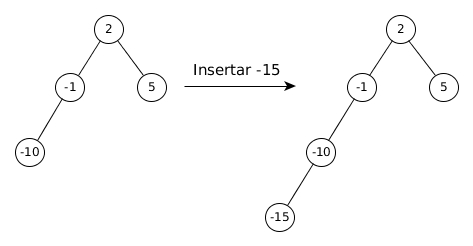
\includegraphics[scale=0.6]{imagenes/fig5.jpg}
	\end{center}
	\caption{desbalanceo de un nodo en una inserci'on}
	\label{fig5}
\end{figure}

\begin{figure}[h]
	\begin{center}
		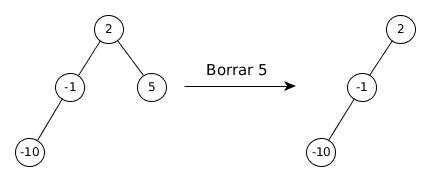
\includegraphics[scale=0.6]{imagenes/fig6.jpg}
	\end{center}
	\caption{desbalanceo de un nodo en un borrado}
	\label{fig6}
\end{figure}


\subsection{Rotaciones en ABBs}

Para remendar los nodos desbalanceados, realizaremos sobre ciertos nodos una serie de operaciones que se conocen como \textit{rotaciones}. Dado que nuestro objetivo es recuperar la condici'on de AVL, necesitamos no s'olo arreglar los factores de balanceo, sino tambi'en mantener el invariante de ABB.

Para restaurar el balanceo, utilizaremos 'unicamente dos tipos de operaciones de rotaci'on, que se ilustran en la figura \ref{fig7}. Notar que estas operaciones son independientes de cualquier noci'on de balanceo, y que son aplicables en cualquier ABB, puesto que preservan el invariante de representaci'on de estos 'arboles. En otras palabras, al aplicar cualquiera de las rotaciones a un ABB, el resultado es otro ABB.

\begin{figure}[H]
	\begin{center}
		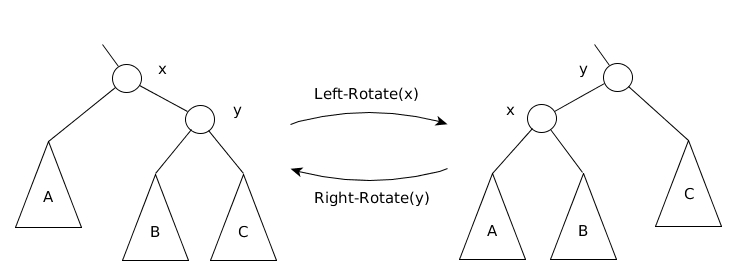
\includegraphics[scale=0.6]{imagenes/fig7.jpg}
	\end{center}
	\caption{rotaciones en ABBs}
	\label{fig7}
\end{figure}

Las dos operaciones son una inversa de la otra. Por un lado, \textsc{Left-Rotate}($x$) toma un nodo $x$, que debe tener un hijo derecho $y$, rotando hacia la izquierda a $x$, dejando a $y$ como ra'iz del sub'arbol, y colgando a la derecha de $x$ el sub'arbol izquierdo de $y$ (si hubiera uno). Observar que al rotar a $x$ a la izquierda, estamos \textit{bajando} a este nodo y \textit{levantando} al nodo $y$.

Por otro lado, \textsc{Right-Rotate}($y$) exige que $y$ tenga un hijo izquierdo, y realiza una operaci'on an'aloga, en forma espejada. En este caso, es al nodo $y$ que rotamos hacia la derecha, haciendo que \textit{baje} y, consecuentemente, que \textit{suba} su hijo izquierdo $x$.

Intuitivamente, utilizaremos \textsc{Left-Rotate}($x$) para trasladar un poco del \textit{peso} del sub'arbol derecho hacia el izquierdo, y \textsc{Right-Rotate}($y$), contrariamente, para llevar peso del sub'arbol izquierdo hacia el derecho. Aqu'i cuando hablamos de peso, no nos referimos a una cantidad de nodos sino a una altura, que es aquello que intentamos balancear.

\subsection{Casos de desbalanceo}

Al realizar una inserci'on o borrado y encontrarnos con que algunos factores de balanceo son estrictamente mayores que 1, resulta conveniente resolver cada uno de estos problemas progresivamente, rebalanceando los nodos m'as profundos, continuando hacia los m'as cercanos a la ra'iz. Por esta raz'on, es 'util plantearse los distintos escenarios en los que tenemos un sub'arbol cuya ra'iz est'a desbalanceada en una unidad (es decir, tiene factor de balanceo -2 'o 2), pero tal que todo otro nodo debajo de dicho nodo est'a balanceado.

Llamemos $p$ a la ra'iz de un tal sub'arbol. Concentr'emonos, primero, en el caso $fb(p) = 2$. Supongamos que el sub'arbol izquierdo de $p$ tiene altura $h$. Entonces, el sub'arbol derecho de $p$ tiene altura $h + 2$. Este sub'arbol derecho debe tener al menos dos nodos, con lo cual podemos nombrar $q$ a su ra'iz. La figura \ref{fig8} muestra la estructura de este 'arbol. A partir de ahora, los n'umeros dentro de cada nodo representar'an los factores de balanceo de los mismos.

\begin{figure}[H]
	\begin{center}
		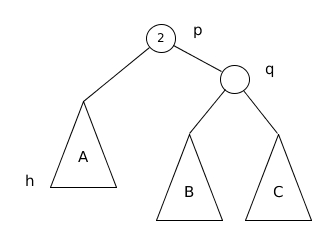
\includegraphics[scale=0.6]{imagenes/fig8.jpg}
	\end{center}
	\caption{$fb(p) = 2$}
	\label{fig8}
\end{figure}

Dividimos nuevamente en casos, seg'un el valor de $fb(q)$. Como asumimos que todos los nodos debajo de $p$ est'an balanceados, debe ser $fb(q) \in \{-1, 0, 1\}$.

Supongamos $fb(q) = 1$. Observar que esto determina las alturas de ambos sub'arboles de $q$. Como el sub'arbol derecho de $p$ es mucho m'as alto que el izquierdo, debemos realizar alg'un tipo de rotaci'on que traslade peso desde la derecha hacia la izquierda. Por este motivo, parece razonable ejecutar una \textsc{Left-Rotate}($p$), y como muestra la figura \ref{fig9}, esta operaci'on reestablece el balance.

\begin{figure}[H]
	\begin{center}
		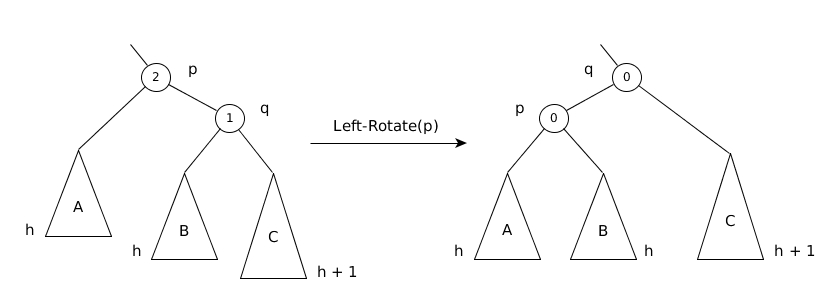
\includegraphics[scale=0.55]{imagenes/fig9.jpg}
	\end{center}
	\caption{$fb(p) = 2$ y $fb(q) = 1$ \textbf{(caso A)}}
	\label{fig9}
\end{figure}

Supongamos $fb(q) = 0$. Utilizando la misma estrategia de rotar $p$ hacia la izquierda, vemos que nuevamente logramos rebalancear el sub'arbol, como muestra la figura \ref{fig10}.

\begin{figure}[H]
	\begin{center}
		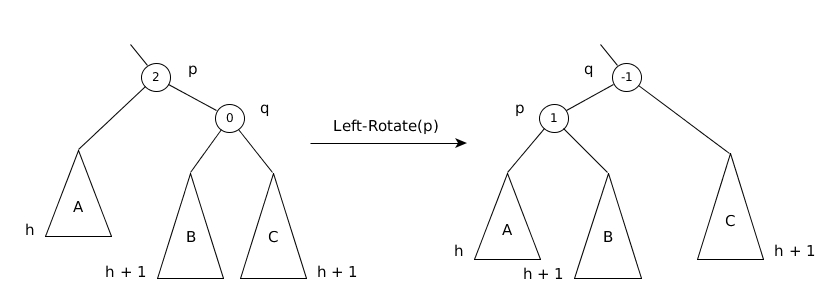
\includegraphics[scale=0.55]{imagenes/fig10.jpg}
	\end{center}
	\caption{$fb(p) = 2$ y $fb(q) = 0$ \textbf{(caso B)}}
	\label{fig10}
\end{figure}

Finalmente, supongamos $fb(q) = -1$. Podemos intentar otra vez la rotaci'on de $p$ hacia la izquierda, aunque lamentablemente esto funciona, pues terminaremos con $fb(q) = -2$, como se ve en la figura \ref{fig11}. Necesitamos rebalancear con m'as cuidado.

\begin{figure}[H]
	\begin{center}
		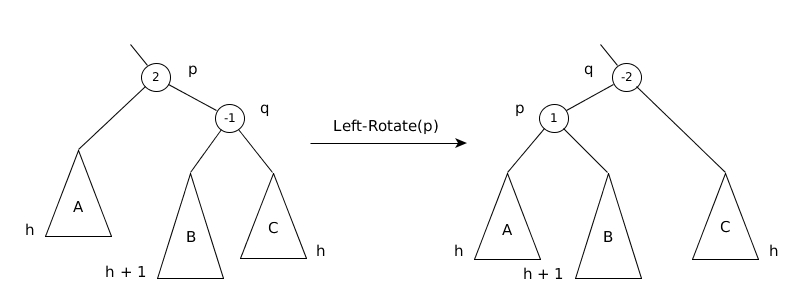
\includegraphics[scale=0.55]{imagenes/fig11.jpg}
	\end{center}
	\caption{rotar $p$ hacia la izquierda falla}
	\label{fig11}
\end{figure}

Notemos que el sub'arbol $B$, que es el m'as pesado de los sub'arboles de $q$, es el que impide llegar al balance. Podemos intentar \textit{desarmar} este 'arbol a trav'es de otras rotaciones, antes de intentar balancear $p$. Como $B$ tiene altura $h + 1$, tiene al menos un nodo, con lo cual podemos llamar $r$ a su ra'iz. La estructura que estamos considerando es la que muestra la figura \ref{fig12}.

\begin{figure}[H]
	\begin{center}
		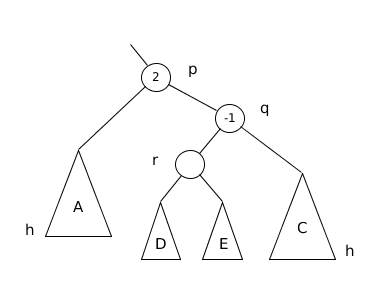
\includegraphics[scale=0.6]{imagenes/fig12.jpg}
	\end{center}
	\caption{$fb(p) = 2$ y $fb(q) = -1$}
	\label{fig12}
\end{figure}

Para distribuir el peso de $B$, necesitamos trasladar una parte de 'el hacia el sub'arbol derecho de $q$. Como podemos intuir a esta altura, es posible conseguir esto v'ia una \textsc{Right-Rotate}($q$). Dejamos como tarea para el lector verificar que esta sola esta rotaci'on puede no ser suficiente en ciertos casos, dependiendo del valor de $fb(r)$. Si ejecutamos la \textsc{Left-Rotate}($p$) pendiente, ahora s'i habremos restaurado el balanceo. El proceso se muestra en la figura \ref{fig13}.

\begin{figure}[H]
	\begin{center}
		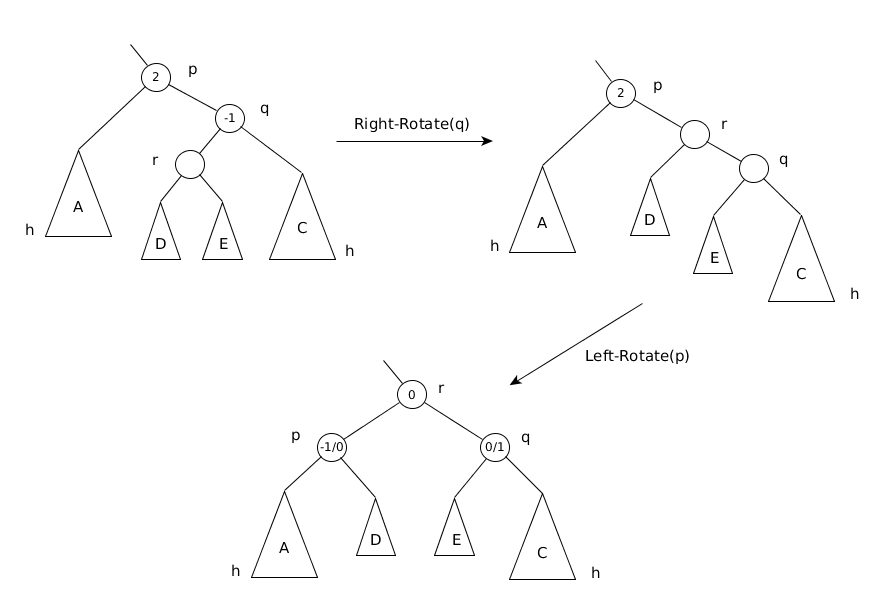
\includegraphics[scale=0.55]{imagenes/fig13.jpg}
	\end{center}
	\caption{$fb(p) = 2$ y $fb(q) = -1$ \textbf{(caso C)}}
	\label{fig13}
\end{figure}

Notemos que los factores de balanceo de $p$ y $q$ depender'an de las alturas de los sub'arboles $D$ y $E$. Si miramos el 'arbol original, el sub'arbol con ra'iz en $r$ ten'ia altura $h + 1$, con lo cual las alturas de $D$ y $E$ son algunas de $h - 1$ 'o $h$.

Hasta ahora estuvimos analizando el caso $fb(p) = 2$. El caso $fb(p) = -2$ es completamente sim'etrico, y no repetiremos el mismo an'alisis detallado. Las figuras \ref{fig14}, \ref{fig15} y \ref{fig16} muestran las rotaciones necesarias para cada uno de los casos, que son, siguiendo el mismo orden que antes, an'alogos.

\begin{figure}[H]
	\begin{center}
		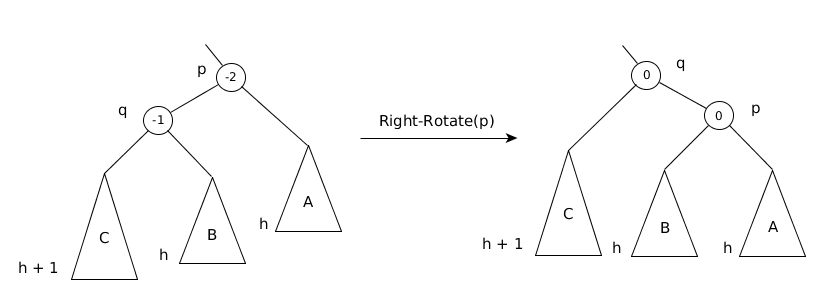
\includegraphics[scale=0.55]{imagenes/fig14.jpg}
	\end{center}
	\caption{$fb(p) = -2$ y $fb(q) = -1$ \textbf{(caso D)}}
	\label{fig14}
\end{figure}

\begin{figure}[H]
	\begin{center}
		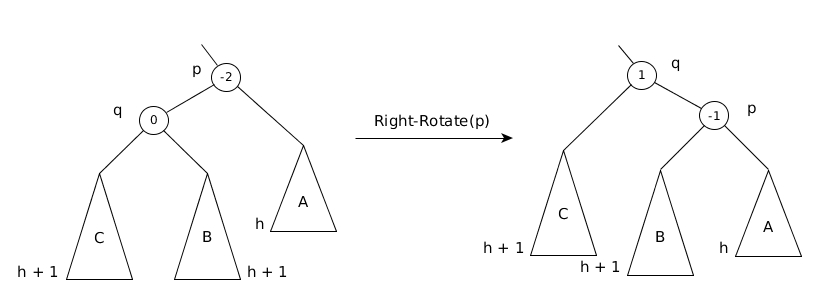
\includegraphics[scale=0.55]{imagenes/fig15.jpg}
	\end{center}
	\caption{$fb(p) = -2$ y $fb(q) = 0$ \textbf{(caso E)}}
	\label{fig15}
\end{figure}

\begin{figure}[H]
	\begin{center}
		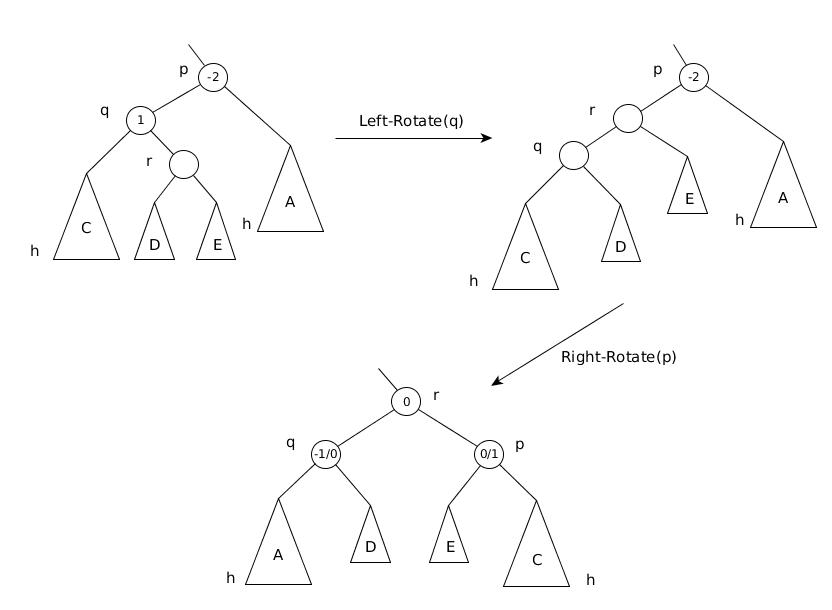
\includegraphics[scale=0.55]{imagenes/fig16.jpg}
	\end{center}
	\caption{$fb(p) = -2$ y $fb(q) = 1$ \textbf{(caso F)}}
	\label{fig16}
\end{figure}

\subsection{Inserci'on en un AVL}

Recordemos que la inserci'on en un AVL agrega un nuevo nodo como una hoja del 'arbol. Esto implica que s'olo pueden cambiar los factores de balanceo de nodos que se encuentren en el camino que entre la ra'iz y el nodo agregado. Si logramos rebalancear cada factor desbalanceado a lo largo de este camino, habremos reestablecido el balance en todo el 'arbol. Esta idea motiva el algoritmo de inserci'on sobre AVLs.

\SetKwFunction{inser}{AVL-Insert}

\begin{algorithm}
  	\DontPrintSemicolon
  	\inser{$T$, $k$}{\;

	\Begin{
		Insertar $k$ en $T$ como en un ABB\;
		Sea $x$ el nodo agregado\;
		\textsc{AVL-Rebalance}($T$, $x$)
 	}
 	}
\end{algorithm}

\SetKwFunction{reba}{AVL-Rebalance}

\begin{algorithm}
  	\DontPrintSemicolon
  	\reba{$T$, $x$}{\;

	\Begin{
		\ForEach {$p$ nodo en el camino entre $x$ y la ra'iz de $T$} {
			\If {$|fb(p)| > 1$} { 
				Rebalancear el sub'arbol con ra'iz en $p$ como en alguno de los casos A, ..., F 
			}
		}
 	}
 	}
\end{algorithm}

La complejidad del algoritmo es claramente proporcional a la altura del 'arbol, es decir, $O(\lg n)$.

La correctitud de este algoritmo se basa fuertemente en que cualquier desbalanceo que nos encontremos tendr'a la forma de alguno de los clasificados anteriormente. Es evidente que el primero de todos que nos encontremos, recorriendo el camino desde abajo, ser'a alguno de los vistos, puesto que el factor de balanceo no puede tener m'odulo mayor que 2, que a su vez se debe a que como s'olo insertamos un nodo, entonces a lo sumo aumentamos la altura de una rama en uno. Pero luego de hacer el primer rebalanceo, ¿por qu'e los factores de nodos superiores no empeoran a'un m'as? ¿No podr'ia pasar que alg'un factor de balanceo pase a tener m'odulo mayor que 2?

Para responder negativamente a esto, debemos analizar c'omo se propagan los cambios en la altura luego de efectuar el primer rebalanceo. Para esto, debemos tener en cuenta c'omo era la altura del sub'arbol a rebalancear, en el instante previo a la inserci'on, y cu'al es su altura luego del rebalanceo.

Hacemos el an'alisis para el rebalanceo del caso A, y dejamos el resto como ejercicio para el lector. 

\begin{teo}
Durante una inserci'on, si el primer rebalanceo es de tipo A, entonces, luego del mismo, ning'un nodo en el camino entre la ra'iz del sub'arbol rebalanceado y la ra'iz de todo el 'arbol tendr'a un factor de balanceo de m'odulo mayor que dos.

\begin{proof}
Utilizamos la notaci'on de la figura \ref{fig9}. Sea $P$ el sub'arbol con ra'iz en $p$, previo a la inserci'on. Sea $Q$ el resultado de insertar y efectuar el primer rebalanceo (de tipo A) en ese sub'arbol. En este caso, la inserci'on se debe haber producido necesariamente en el sub'arbol $C$ (¿por qu'e?), y la altura de $P$ es $h + 2$. Como la altura de $Q$ tambi'en es $h + 2$, entonces ning'un factor de balanceo de un nodo en el camino entre la ra'iz de $Q$ y la ra'iz del 'arbol pudo haber cambiado respecto de su valor previo a la inserci'on.
\end{proof}
\end{teo}

Observar que este resultado muestra algo m'as fuerte que lo que quer'iamos. Hemos probado que, en una inserci'on, si el primer rebalanceo es de tipo A, luego del mismo todo el 'arbol queda balanceado. Se puede demostrar que, luego de una inserci'on, los 'unicos casos de rebalanceo que se pueden dar son A, C, D y F, y que luego de realizar alguno de ellos, todos los factores de balanceo quedan reestablecidos.

\subsection{Borrado en un AVL}

Recordemos que los casos de borrado en un ABB son tres, que dependen de la cantidad de hijos del nodo a borrar. Llamemos $z$ al nodo a borrar.

Si $z$ no tiene hijos, entonces es borrado y el resto del 'arbol no cambia. Esto s'olo puede generar variaciones de a lo sumo una unidad en los factores de balanceo de los nodos del camino entre el padre de $z$ y la ra'iz.

Si $z$ tiene un 'unico hijo, entonces ese hijo es conectado con el padre de $z$. Al igual que antes, s'olo pueden cambiar en uno, los factores de nodos entre el padre de $z$ y la ra'iz.

Por 'ultimo, si $z$ tiene dos hijos, $z$ es reemplazado por el nodo antecesor (o el sucesor) en el sub'arbol del cual es ra'iz. En otras palabras, se reemplaza $z$ por el nodo de clave m'axima en su sub'arbol izquierdo, al que llamamos $x$, y al 'unico hijo de $x$ se lo conecta con el padre de $x$, salvo cuando $x$ es el hijo izquierdo de $z$, en cuyo caso el hijo de $x$ conservar'a su relaci'on con $x$. Por ende, s'olo cambiar'an los factores de balanceo de los nodos entre el antiguo padre de $x$ (si $x$ no es hijo de $z$) o bien $x$ mismo (en caso contrario), y la ra'iz del 'arbol.

Este argumento muestra que, al igual que en la inserci'on, el borrado de nodos s'olo modifica, a lo sumo en una unidad, los factores de balanceo de nodos entre cierto nodo particular (que depende del caso de borrado) y la ra'iz.

%\newpage

\SetKwFunction{dele}{AVL-Delete}

\begin{algorithm}
  	\DontPrintSemicolon
  	\dele{$T$, $k$}{\;

	\Begin{
		Borrar $k$ de $T$ como en un ABB\;
		Sea $x$ primer nodo posiblemente desbalanceado\;
		\textsc{AVL-Rebalance}($T$, $x$)
 	}
 	}
\end{algorithm}

El costo de este algoritmo tambi'en es proporcional a la altura del 'arbol, o sea, $O(\lg n)$.

Al igual que en la inserci'on, el algoritmo se basa en que nunca aparecer'a un nodo desbalanceado con un factor de balanceo de m'odulo mayor que 2, pero no daremos una prueba formal de que esto efectivamente ocurre.

En el caso del borrado, cualquiera de los seis casos de rebalanceo puede darse, y el desbalance puede propagarse hacia nodos superiores, a'un luego de haber efectuado una operaci'on de rebalanceo. Por este motivo, no es posible cortar anticipadamente el recorrido hacia la ra'iz, luego del primer rebalanceo, como s'i era posible en la inserci'on.
